% Tor Vergata - Engineering Beamer template.
% Roberto Masocco <robmasocco[at]gmail.com>
% Alessandro Tenaglia <alessandro.tenaglia42[at]gmail.com>
% First version: February 5, 2022
% Last update: November 16, 2024

% Preferred aspect ratio is 16:9 but feel free to change it here
\documentclass[aspectratio=169]{beamer}

% Customized document information by setting these string options
% To leave a field empty, use "{}"
% If you want to hide navigation symbols, go to line 144 of the style file
\usepackage[
    title={The Alexandrov Moving Planes Method\\ and Applications to Geometric Flows},
    subtitle={},
    event={Tesi di Laurea Magistrale},
    author={Marco Tamburro},
    longauthor={Marco Tamburro},
    email={marco.tamburro@students.uniroma2.eu},
    institute={Tor Vergata},
    longinstitute={Università degli studi di Roma Tor Vergata},
    department={Relatore: Prof. Carlo Sinestrari},
    researchgroup={},
    date={11 Dic 2024}
]{utvengbeamer}
\usepackage{comment}
\usepackage{amsmath}
\usepackage{amsfonts}
\usepackage{amssymb}
\usepackage{amsthm}
\usepackage{array}
\usepackage{mathtools}

\begin{document}
\graphicspath{{figs/}}
% --- Title page ---
\frame{\titlepage}


% Include sections here, like this
% --- Section 1 ---
% !TeX spellcheck = it_IT
% --- Equazione di cui ci occupiamo ---
\begin{frame}{Equazione di cui ci occupiamo}{}
	\begin{block}{Flusso geometrico di cui ci occupiamo}
		$X_0$ varietà differenziabile \textit{embedded} in $\mathbb{R}^{n+1}$, la facciamo evolvere secondo
		\begin{align*}
				\frac{\partial X_t}{\partial t} = - F(\kappa_1(x), \dots , \kappa_n(x)) \nu
		\end{align*}
		dove $\nu$ è il vettore normale, $\kappa_i$ le curvature principali e $F$ una funzione simmetrica tale che 
		\begin{align*}
			\frac{\partial F}{\partial \kappa_i} > 0 \mathrm{\; for \; all } \; i=1,\dots, n
		\end{align*}
	\end{block}
	%\begin{block}<2->
		%Quello di cui voglio convincervi con questa presentazione è che le soluzioni di questo flusso diventano più \textit{tonde} e \textit{simmetriche} andando avanti nel tempo
	%\end{block}
\end{frame}


\section{Introduzione}

% --- Struttura della tesi ---
\begin{frame}{Struttura della tesi}{}

\begin{itemize}
	\item \textbf{Capitolo 1}: richiami e risultati preliminari 
	\item \textbf{Capitolo 2}: introduzione del metodo dei piani di Alexandrov in $\mathbb{R}^n$, $\mathbb{H}^n$, $S^n$
	\item \textbf{Capitolo 3}: dimostrazione del teorema di Chow-Gulliver e conseguenze in $\R^n$
	\item \textbf{Capitolo 4}: estensione del teorema di Chow-Gulliver ad $\mathbb{H}^n$ ed $S^n$ 
	\item \textbf{Capitolo 5}: flussi che preservano l'area e il volume
\end{itemize}
\end{frame}


% --- Table of contents ---
\begin{frame}
	\frametitle{Struttura della presentazione}
	\tableofcontents
\end{frame}

% --- Di cosa parliamo ---
\begin{comment}{Di cosa parliamo oggi}{}
\begin{itemize}
	\item Alexandrov Moving Planes Method
	\item Il risultato di Chow-Gulliver
	\item Alcune conseguenze e corollari
	\item Cenni sull'estensione a spazi a curvatura costante
\end{itemize}
\end{comment}



% --- Di cosa *non* parliamo ---
%\begin{frame}{Di cosa \textbf{non} parliamo oggi}{(ma che è nella tesi)}
%
	%\begin{itemize}
		%\item Dettagli e dimostrazioni (oltre a qualche cenno sul teorema principale)
		%\item Discussioni approfondite sugli spazi a curvatura costante
		%\item Flussi che preservano l'area e il volume
	%\end{itemize}
%\end{frame}


% --- Section 2 ---
% !TeX spellcheck = it_IT
\section{Alexandrov Moving Planes Method}
% --- Moving planes ---
\begin{frame}{Alexandrov Moving Planes Method}{Cenni storici}
	\begin{itemize}
		\item Tecnica per dimostrare la simmetria delle soluzioni a PDE ellittiche e paraboliche. 
		\item<2-> Introdotto da Alexandrov per caratterizzare la sfera 
		\begin{itemize}
			\item Alexandrov A.D.; \textit{A characteristic property of spheres}, 1962
		\end{itemize}
		\item<3-> Serrin e da Gidas-Ni-Nirenberg lo applicano a soluzioni di PDE ellittiche di natura non-geometrica
		\begin{itemize}
			\item Serrin J.; \textit{A symmetry problem in potential theory}, 1971
			\item Gidas B., Ni W.M., Nirenberg L.; \textit{Symmetry and Related Properties via the Maximum Principle}, 1979
		\end{itemize}
	\end{itemize}
\end{frame}

% --- Moving planes ---
\begin{frame}{Alexandrov Moving Planes Method}{Il metodo in breve}
	\begin{columns}
		% First column
		\column{.72\textwidth}
		\begin{itemize}
			\item Rifletto una soluzione rispetto a una famiglia di piani paralleli
			\item<2-> Considero il piano dove c'è ``per la prima volta'' \textit{tangenza interna} dei grafici
			\item<3-> Applico il principio del massimo alla differenza di soluzione e riflessione
			\item<4-> Deduco che la funzione è simmetrica rispetto a quel piano. Per arbitrarietà della direzione, ho simmetria sferica
		\end{itemize}
		% Second column
		\column{.28\textwidth}
		\begin{figure}
			\begin{center}
				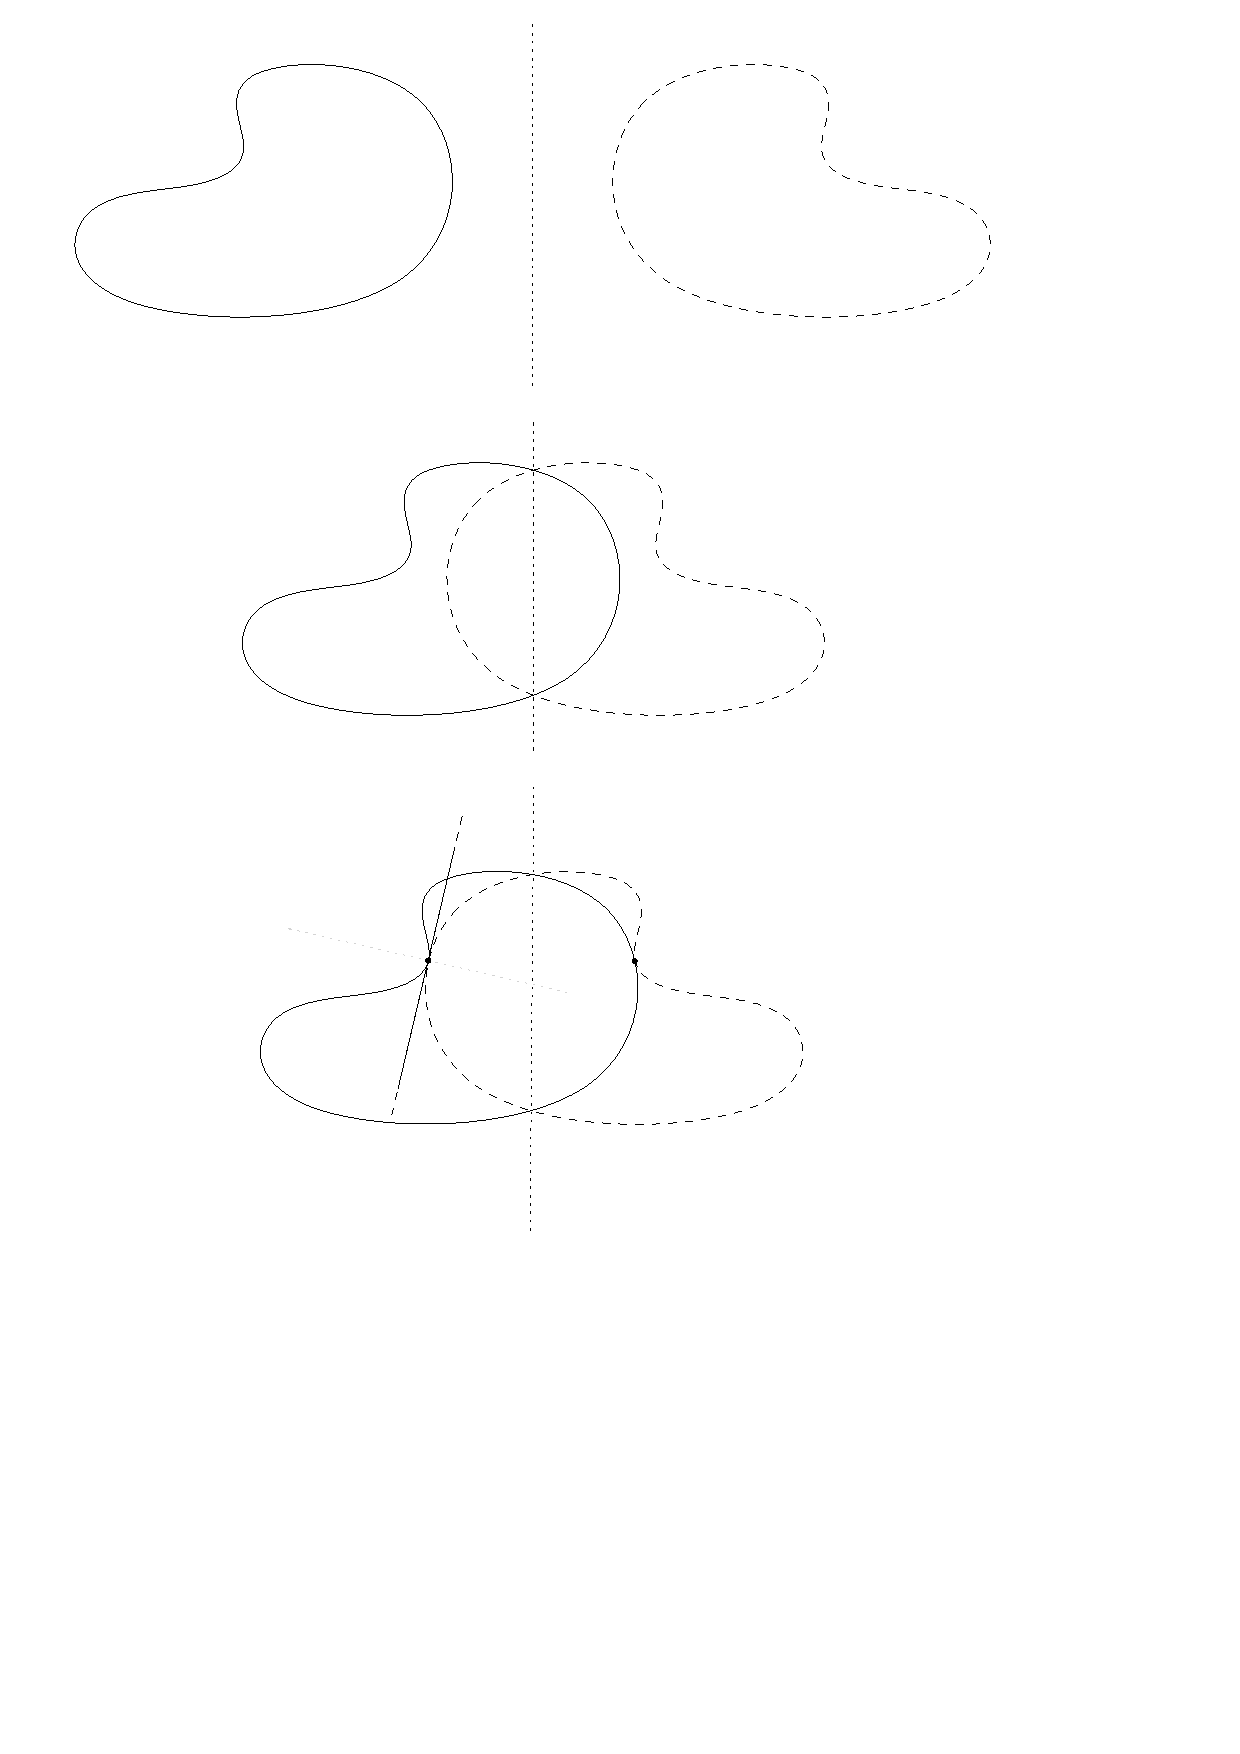
\includegraphics[width=\textwidth]{6_method moving planes}
				\caption{}
			\end{center}
		\end{figure}
	\end{columns}
\end{frame}

\section{Il risultato di Chow-Gulliver}


% --- Equazione di cui ci occupiamo ---
\begin{frame}{Equazione di cui ci occupiamo}{}
	\begin{block}{Flusso geometrico di cui ci occupiamo}
		\begin{align*}
			\frac{\partial X_t}{\partial t} = - F(\kappa_1(x), \dots , \kappa_n(x)) \nu
		\end{align*}
		dove $\nu$ è il vettore normale, $\kappa_i$ le curvature principali e $F$ una funzione simmetrica tale che 
		\begin{align*}
			\frac{\partial F}{\partial \kappa_i} > 0 \mathrm{\; for \; all } \; i=1,\dots, n
		\end{align*}
	\end{block}
	\begin{block}{}<2->
		La condizione sulle derivate di $F$ è equivalente a dire che questa sia una \textbf{equazione parabolica} (non-lineare). In particolare, possiamo applicare il principio del massimo e l'Hopf Boundary Point Lemma alla differenza di due soluzioni. Inoltre, la parabolicità garantisce l'esistenza per tempi piccoli.
	\end{block}
\end{frame}



% --- Riflessione stretta ---
\begin{frame}{Riflessione stretta}{Definizione}
	\begin{block}{Riflessione stretta}
		 Possiamo riflettere $X : M^n \rightarrow R^{n+1}$ strettamente rispetto a $\pi$ se entrambe le seguenti cose sono vere:
		 \begin{itemize}
		 	\item La riflessione di $X$ rispetto a $\pi$ nel semispazio delimitato da $\pi$ resta dentro l'altra metà di $X$, toccandosi solo sul piano
		 	\item A tutti i punti sul piano, $X$ e la sua riflessione rispetto a $\pi$ non hanno lo stesso vettore normale su $\pi$
		 \end{itemize}
	\end{block}
\end{frame}


% --- Cosa non deve succedere ---
\begin{frame}{Riflessione stretta}{Cosa non deve succedere}
	\begin{columns}
		% First column
		\column{.5\textwidth}
		\begin{figure}
			\begin{center}
				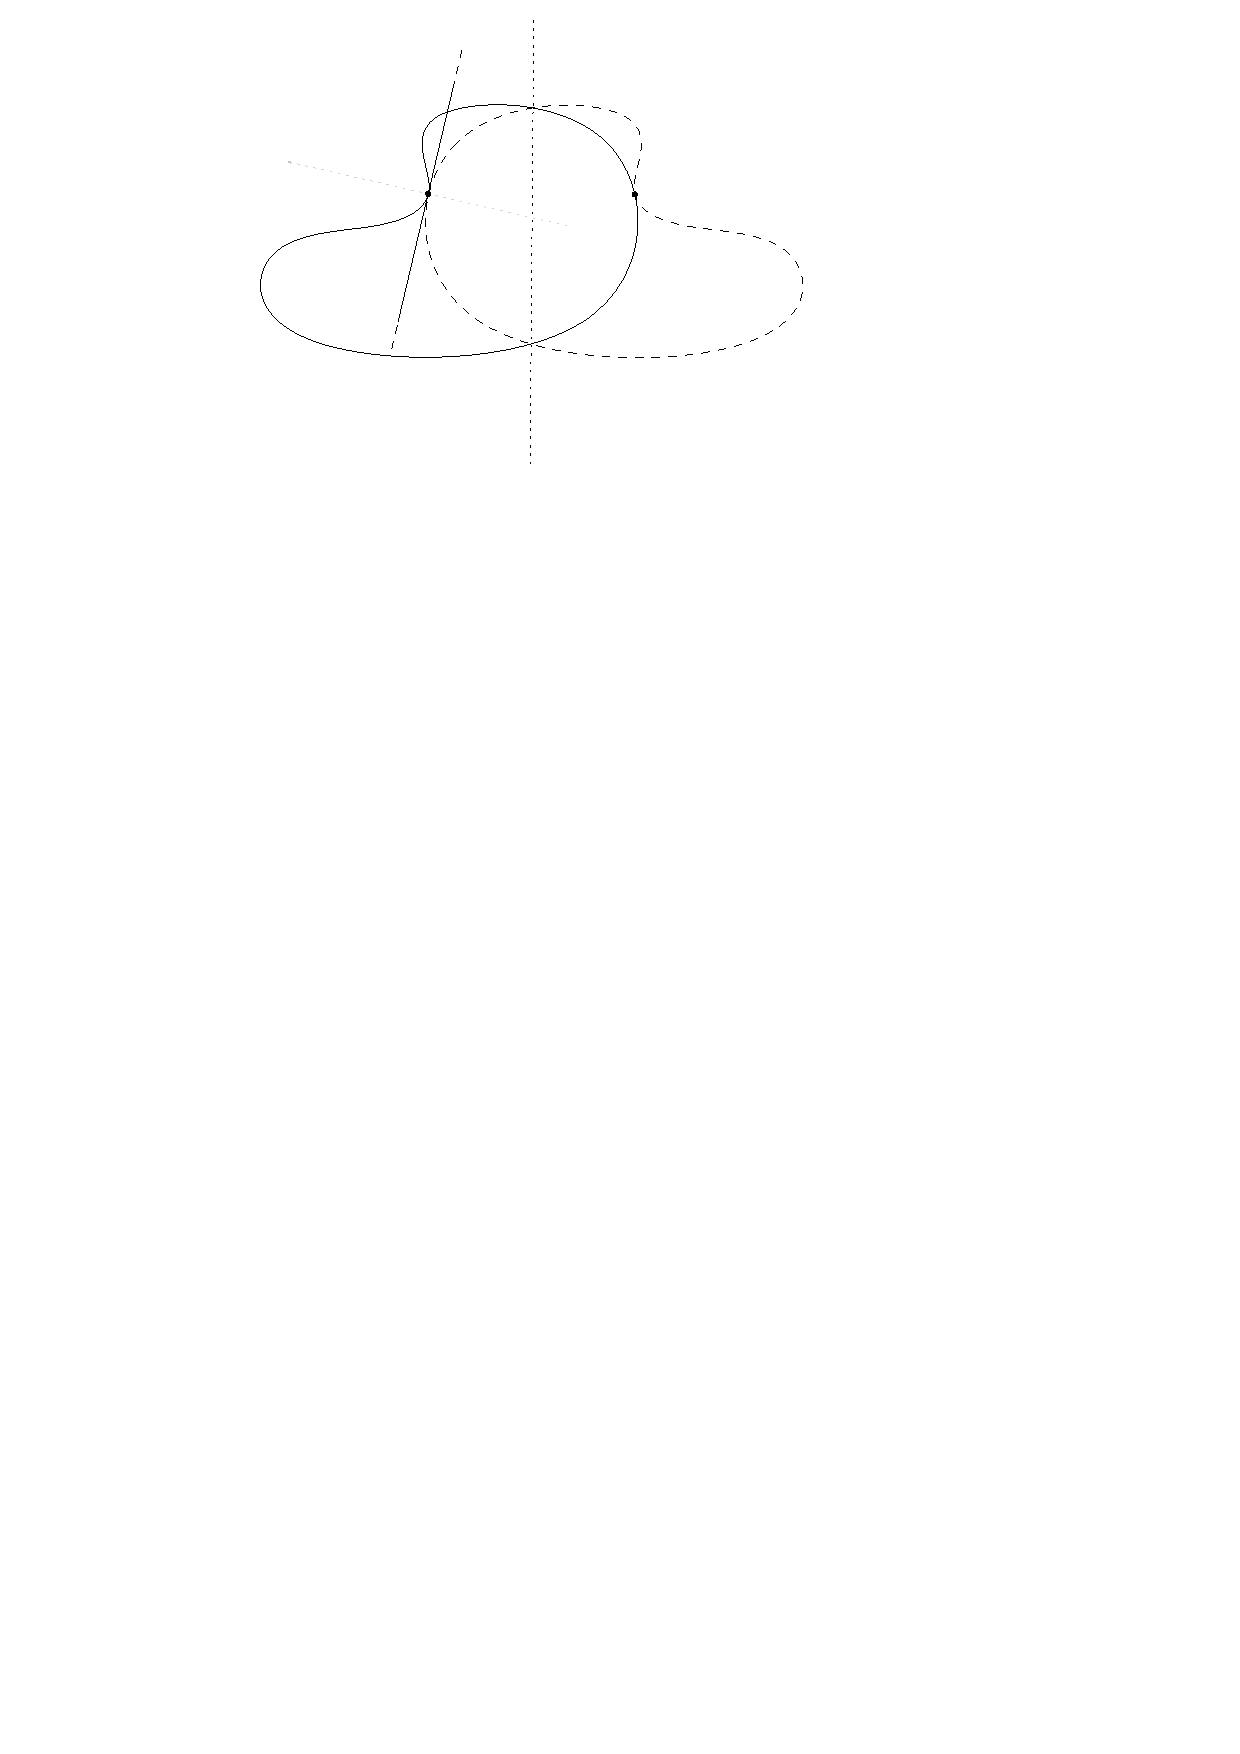
\includegraphics[width=0.8\textwidth]{8_interior_contact}
				\caption{Esempio di contatto interno}
			\end{center}
		\end{figure}
		% Second column
		\column{.5\textwidth}
		\begin{figure}
			\begin{center}
				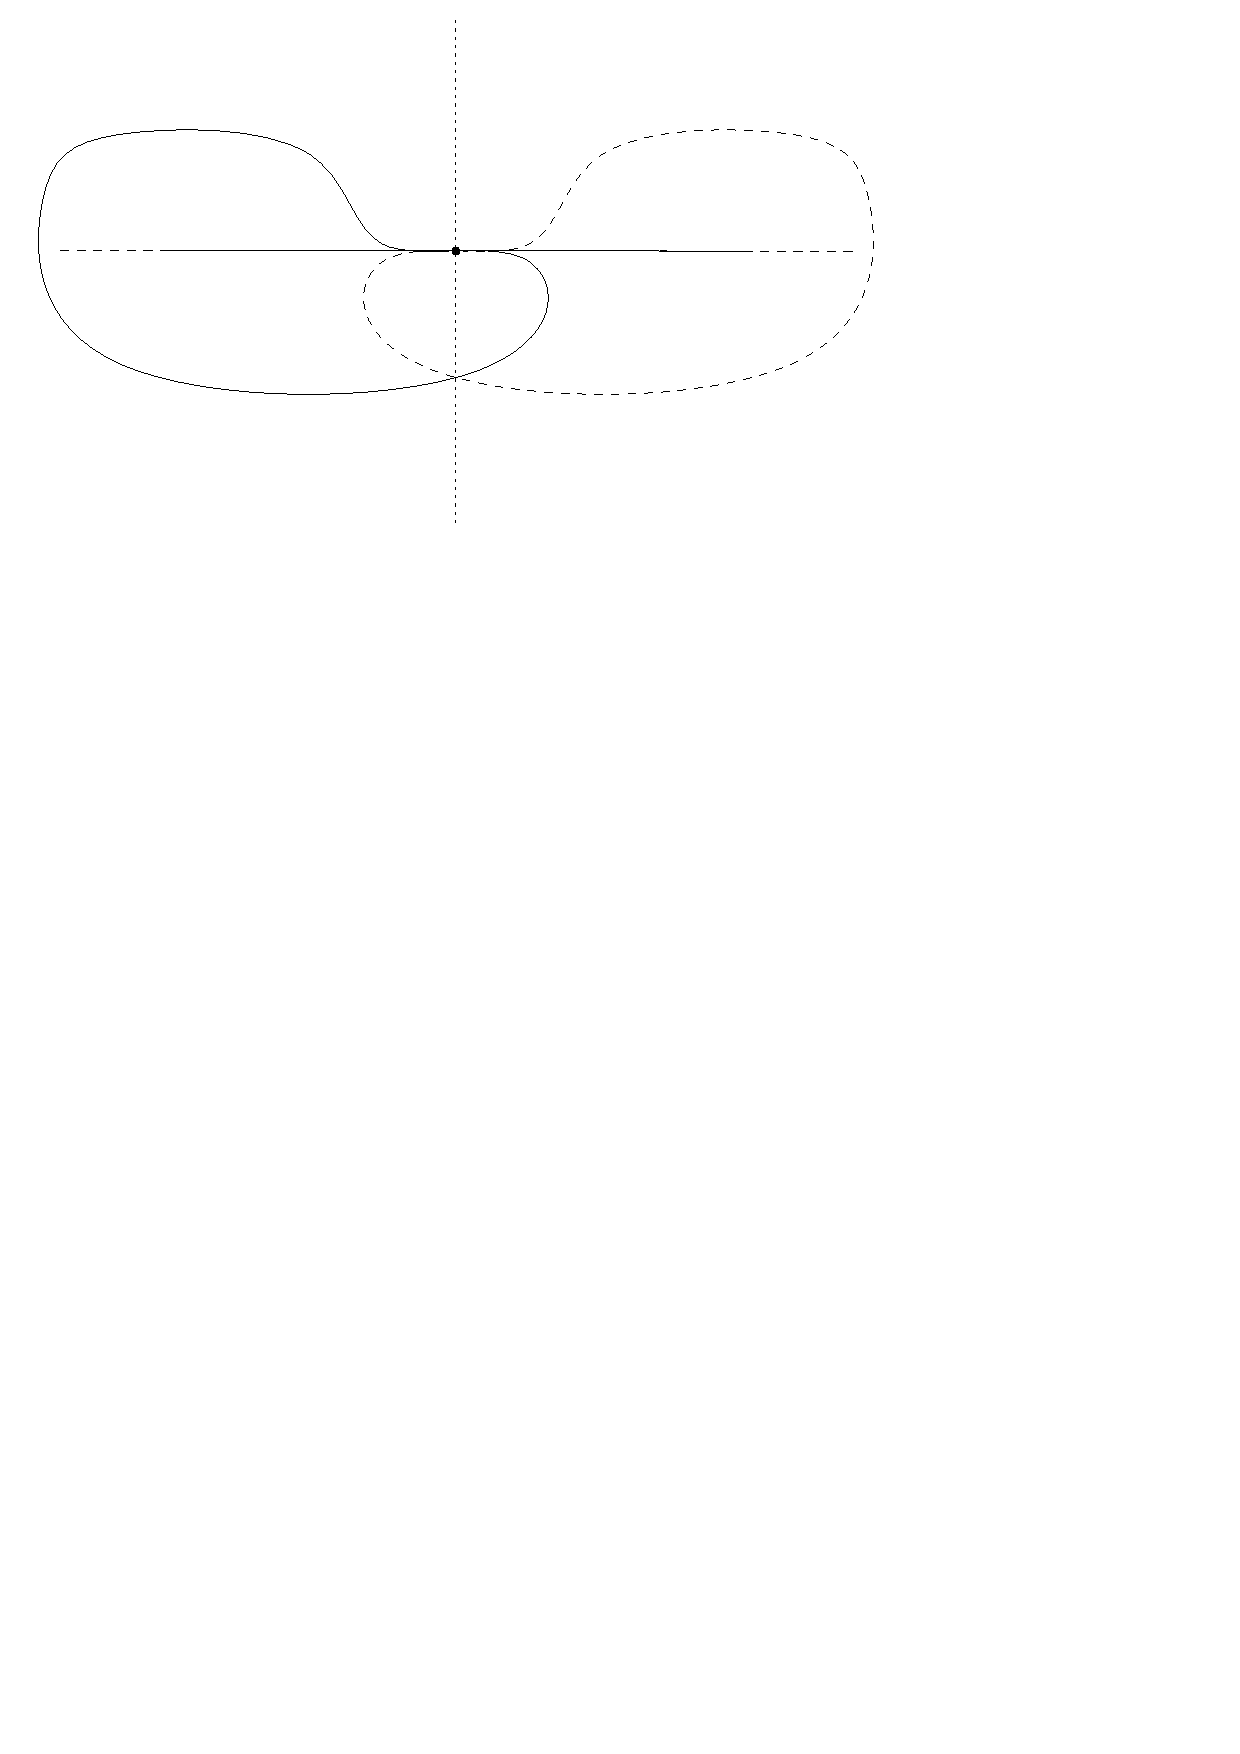
\includegraphics[width=\textwidth]{9_boundary_contact}
				\caption{Esempio di contatto al bordo}
			\end{center}
		\end{figure}
	\end{columns}
\end{frame}




% --- Il teorema di Chow e Gulliver ---
\begin{frame}{Il teorema di Chow e Gulliver}{}
	\begin{block}{Teorema (Chow-Gulliver)}
		Data una soluzione del flusso che stiamo considerando, se possiamo riflettere il dato iniziale $X_0$ strettamente rispetto ad un piano $\pi$, allora possiamo riflettere $X_t$ strettamente rispetto a $\pi$ per ogni $t\in [0,T)$ (intervallo in cui è definita la soluzione). 
	\end{block}
	\begin{block}{}<2->
		\textbf{Interpretazione intuitiva}: i piani rispetto a cui posso riflettere \textit{aumentano} nel tempo, per cui la varietà diventa \textit{più simmetrica} e tonda. 
	\end{block}
\end{frame}
% --- Section 3 ---
% !TeX spellcheck = it_IT
\section{Due esempi di corollari}

% --- Il teorema di Chow e Gulliver ---
\begin{frame}{Due corollari}{}
	\begin{block}{Corollario (Chow)}<1->
		Data una soluzione $C^2$ al problema, esiste $C$, \textbf{che dipende solo dal dato iniziale}, tale che ad ogni istante $t$:
		\begin{equation}
			\max_{x\in X_t} |x| - \min_{x\in X_t} |x| <C
		\end{equation}
	\end{block}
	\begin{block}{}<2->
		Se considero la soluzione riscalata, $\frac{X_t}{\max_{x\in X_t} |x|}$, per un flusso espansivo dove $\lim_{t\rightarrow T}\max_{x\in X_t} |x| = +\infty$, converge a una sfera 
	\end{block}
	\begin{block}{Corollario (Risa-Sinestrari)}<3->
		Non esistono soluzioni antiche espansive ($F<0$) che \textit{escono fuori da un punto} oltre alle sfere. 
	\end{block}
\end{frame}

\section{Cenni sulla parte originale della tesi}
% --- Frame: text and figure ---
\begin{frame}{Estensione a spazi a curvatura costante}{Idea}
	\begin{columns}
		% First column
		\column{.5\textwidth}
		Il risultato di Chow e Gulliver si estende al caso in cui lo spazio ambiente è $\mathbb{H}^{n+1}$ o $S^{n+1}$. 
		\begin{itemize}
			\item<1-> L'equazione continua ad essere parabolica anche negli spazi a curvatura costante
			\item<2-> Introduciamo una notazione che consente di impostare il problema
			\item<3-> La dimostrazione di Chow-Gulliver può essere estesa
		\end{itemize}
		% Second column
		\column{.5\textwidth}
		\begin{figure}
			\begin{center}
				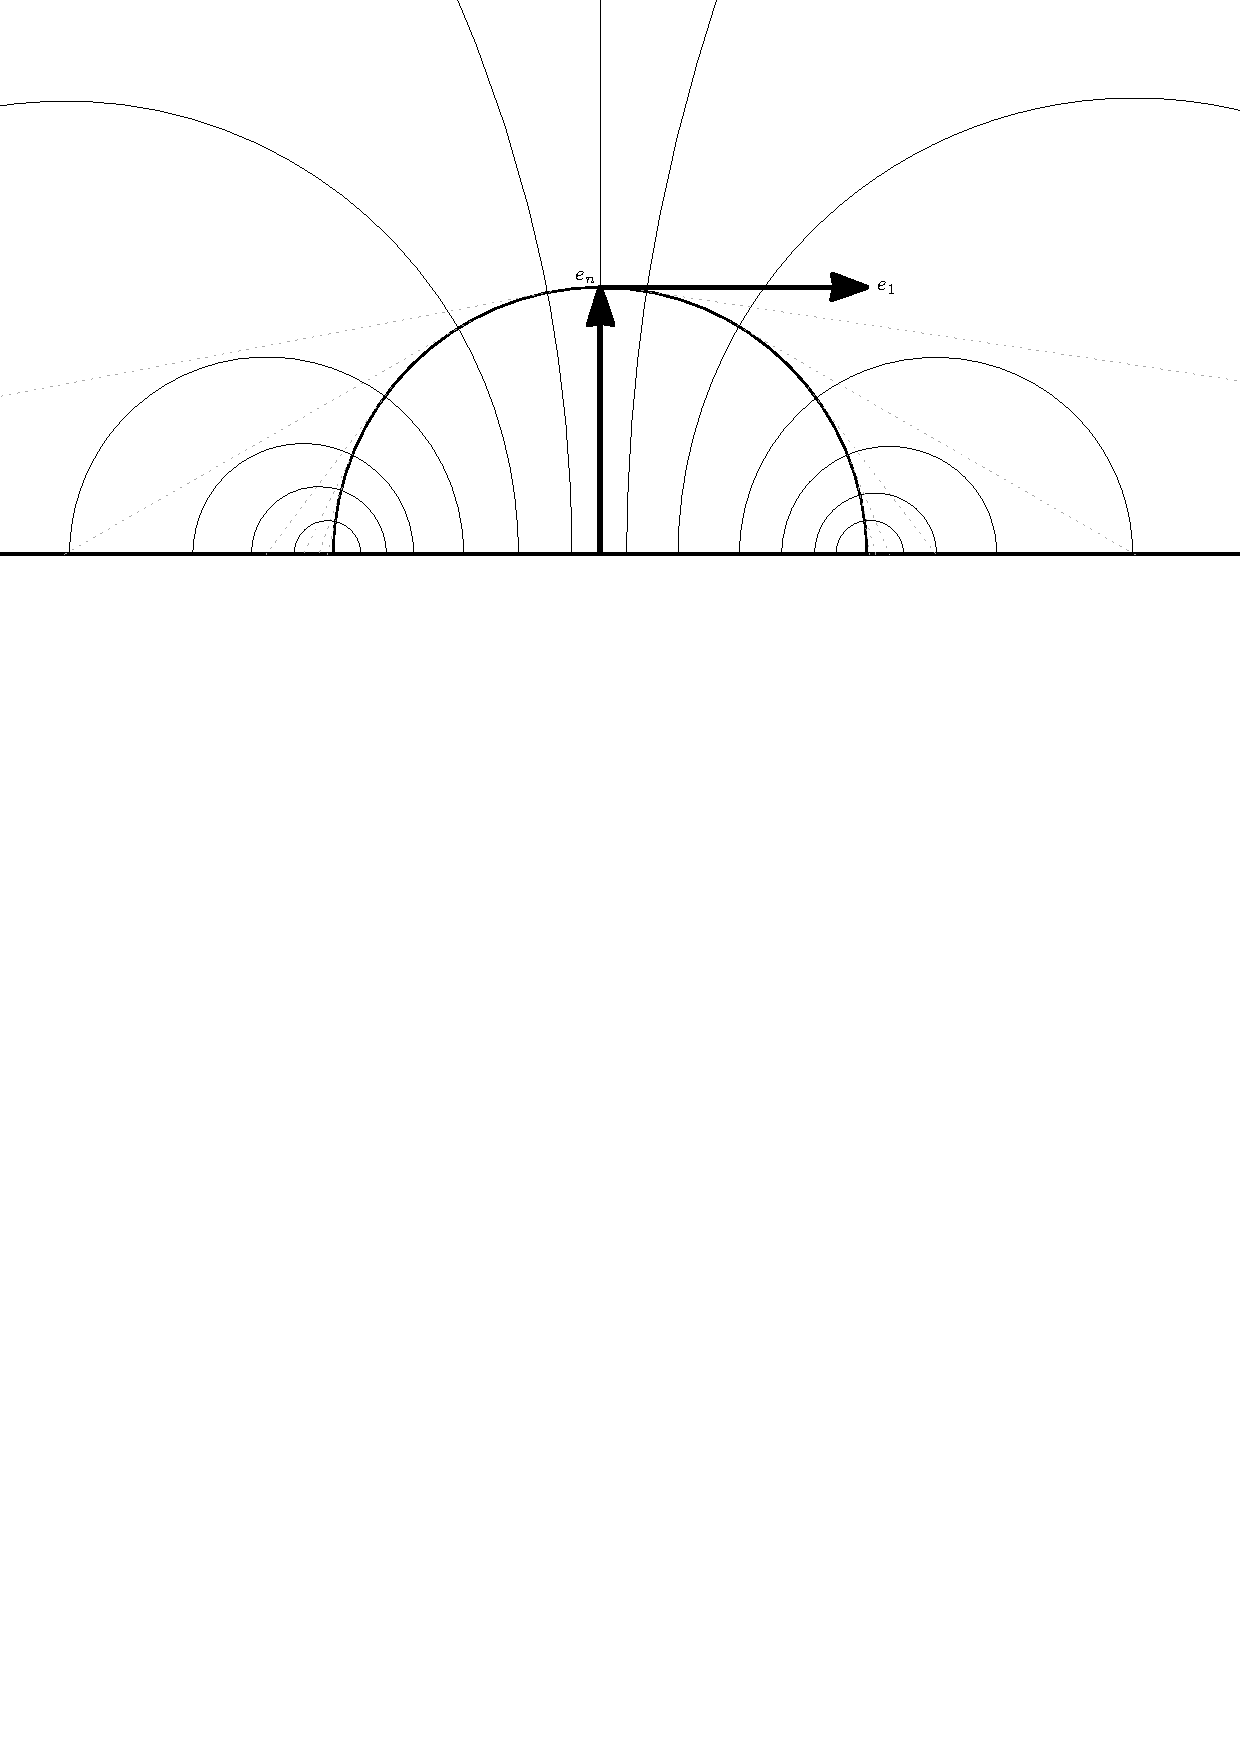
\includegraphics[width=\textwidth]{5b_moving_planes_hyperbolic}
				\caption{Iperpiani totalmente geodetici perpendicolari a una data geodetica in $\mathbb{H}^2$}
			\end{center}
		\end{figure}
	\end{columns}
\end{frame}

% --- Frame: text and figure ---
\begin{frame}{Estensione a spazi a curvatura costante}{Differenze con il caso euclideo}
	\begin{columns}
		% First column
		\column{.5\textwidth}
		\begin{itemize}
			\item<1-> Iperpiani sostituiti da superfici totalmente geodetiche
			\item<2-> Anche dimostrare che delle riflessioni esistono non è più banale
			\item<3-> Non è più ben definito un concetto di parallelismo tra gli iperpiani 
			\begin{itemize}
				\item Nel metodo consideriamo quelli ortogonali a una geodetica, ma non restano equidistanti in tutti i punti
			\end{itemize}
			\item<4-> Il trasporto parallelo non è banale
		\end{itemize}
		% Second column
		\column{.5\textwidth}
		\begin{figure}
			\begin{center}
				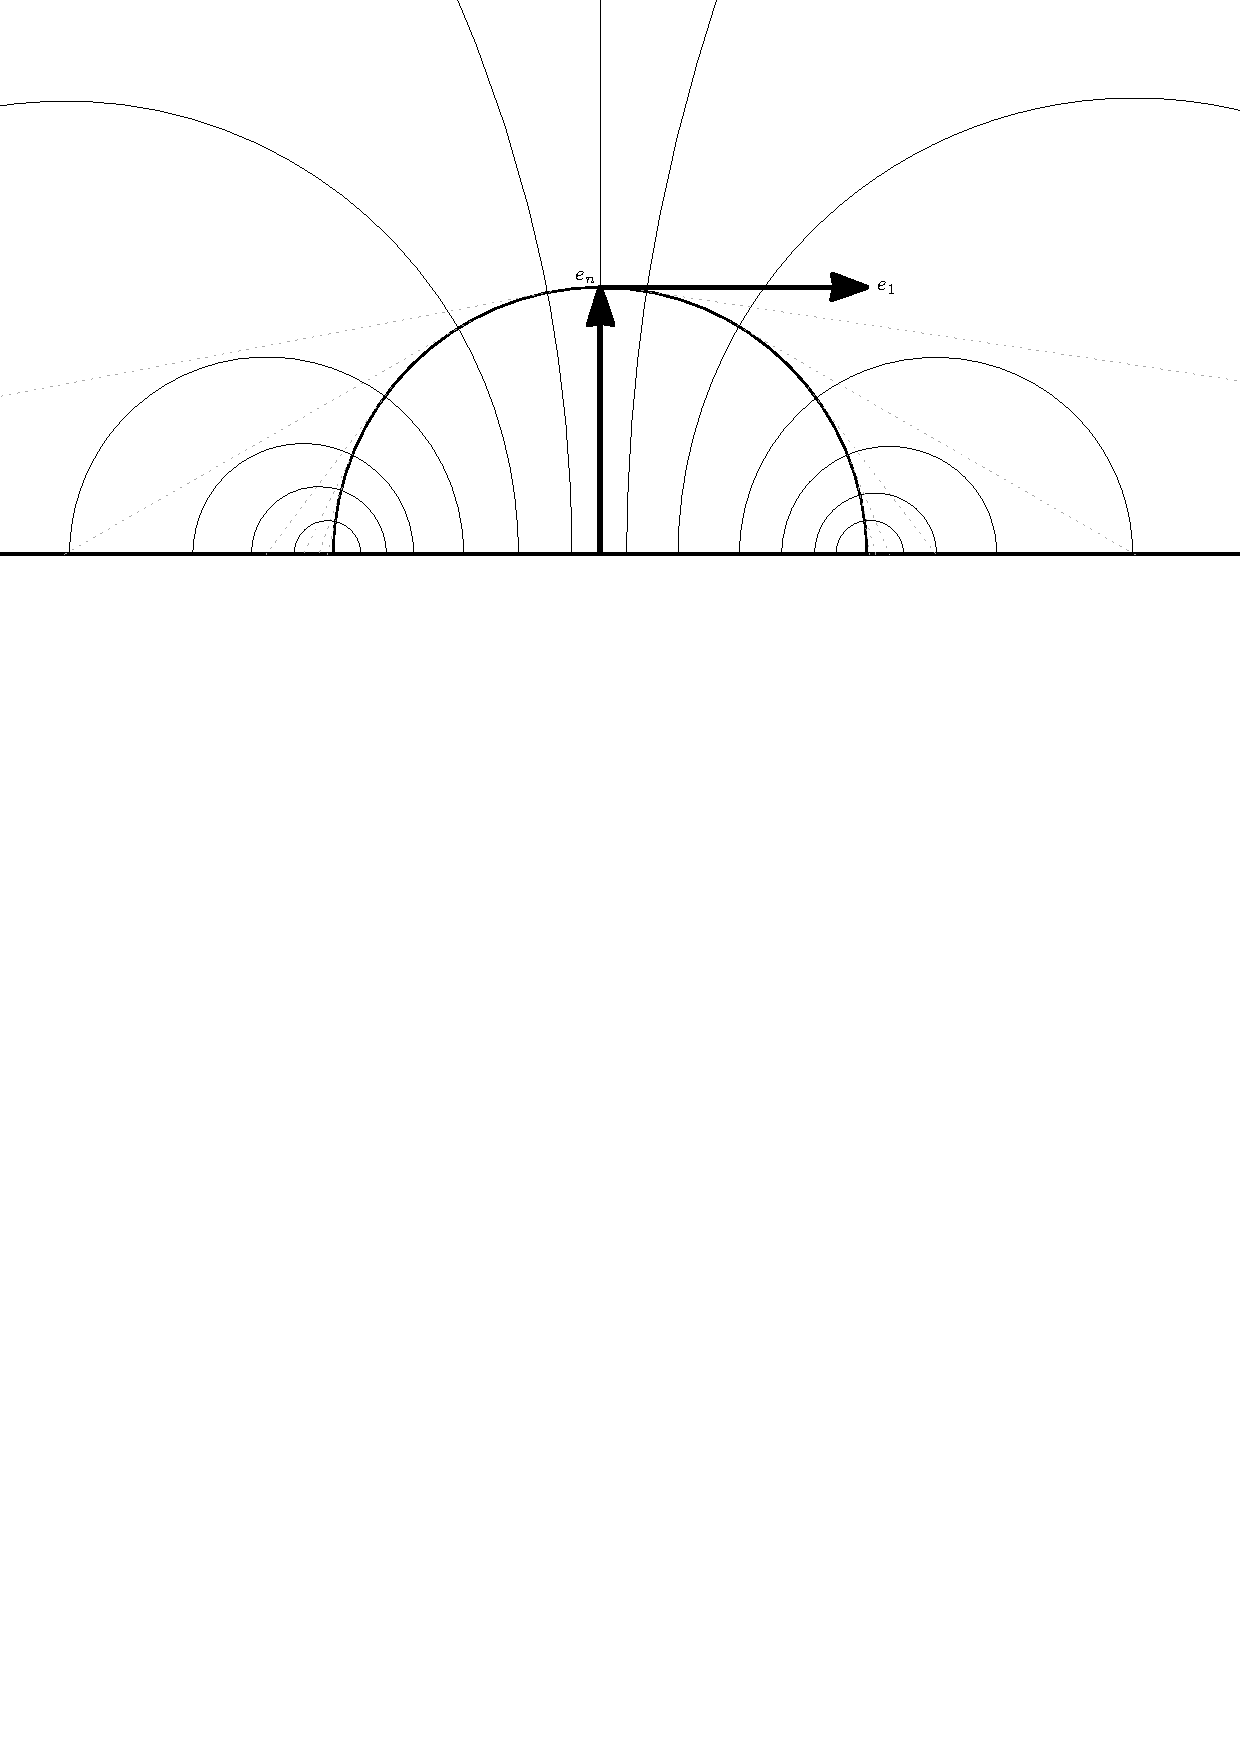
\includegraphics[width=\textwidth]{5b_moving_planes_hyperbolic}
				\caption{Iperpiani totalmente geodetici perpendicolari a una data geodetica in $\mathbb{H}^2$}
			\end{center}
		\end{figure}
	\end{columns}
\end{frame}


% --- Frame: text and figure ---
\begin{frame}{Estensione a spazi a curvatura costante}{Corollari}
	Alcuni corollari continuano a valere, ad esempio resta vero che 
	\begin{block}{Corollario}
		Non esistono soluzioni antiche espansive ($F<0$) che \textit{escono fuori da un punto} oltre alle sfere (intese come luogo dei punti equidistanti da un'origine). 
	\end{block}
\end{frame}


% --- Frame: text and figure ---
\begin{frame}{Estensione a spazi a curvatura costante}{Corollari}
	Alcuni corollari continuano a valere, ad esempio resta vero che 
	\begin{block}{Corollario}
		Non esistono soluzioni antiche espansive ($F<0$) che \textit{escono fuori da un punto} oltre alle sfere (intese come luogo dei punti equidistanti da un'origine). 
	\end{block}
	%Sulla sfera esiste anche una specie di risultato inverso di altri autori, dimostrato con altre tecniche di riflessione:
	%\begin{block}{Corollario}
		%Per una soluzione \textit{contrattiva} e \textit{convessa}, definita sul massimo intervallo possibile e dove il $\lim \sup$ della curvatura media è finita, allora il flusso è composto da sfere che si contraggono
	%\end{block}
\end{frame}



% --- Equazione di cui ci occupiamo ---
\begin{frame}{Flussi ad area e volume costante}{}
	\begin{block}{Flusso ad area/volume costante}
		\begin{align*}
			\frac{\partial X_t}{\partial t} = \left(-\frac{\sum_i \kappa_i(x)}{n}+\phi(t)\right) \nu
		\end{align*}
		consideriamo il flusso dove $F$ è la curvatura media $H$, e aggiungiamo un termine globale che lo rende a area/volume costante. Per conservare il volume: 
		\begin{align*}
			\phi(t) = \frac{\int_{X_t} H^2(x, t) \, d\mu}{\int_{X_t} H(x, t) \, d\mu}
		\end{align*}
	\end{block}
	\begin{block}{}<2->
		Il teorema di Chow e Gulliver si estende anche a questa classe di flussi
	\end{block}
	\begin{block}{}<3->
		Usando il metodo è possibile dimostrare che il flusso non esce fuori da un compatto
	\end{block}
\end{frame}


% --- Section 3 ---
% !TeX spellcheck = it_IT
\section{Riassunto}
% --- Riassunto ---
\begin{frame}{Riassunto}{}
	\begin{itemize}
		\item Il metodo dei piani di Alexandrov è una tecnica che consente di dimostrare simmetrie radiali per soluzioni di un'ampia classe di PDE
		\item<2-> Una ampia classe di flussi geometrici è parabolica, e a questi si può applicare un risultato di \textit{monotonia delle simmetrie} di Chow e Gulliver
		\item<3-> La tecnica è estremamente versatile e consente di dimostrare facilmente molti risultati apparentemente difficili
		\item<4-> I risultati principali possono essere estesi anche nel caso di spazi a curvatura costante e a flussi \textit{modificati} per conservare il volume interno o l'area
	\end{itemize}
\end{frame}

\frame{\titlepage}




% Include sections here, like this
% --- Section 1 ---
%\input{sections/section1}

% --- Section 2 ---
%\input{sections/section2}

\end{document}
